\section{Higher harmonic generation microscopy}
Higher harmonic generation is a nonlinear scattering process resulting from light interacting with tissue.
Photons from the incident laser beam combine into one photon via a virtual state, preserving the energy.
In this study, two higher harmonic generation variants are used: second and third harmonic generation (SHG and THG, respectively).
THG happens at structural interfaces, making it useful to image \eg cells and their nuclei, or axons.
SHG is generated by non-centrosymmetric structures, such as collagen and microtubules.
Some molecules fluoresce, producing a photon with slightly less energy than the incoming photons.
The difference in energy goes into non-radiative processes, including vibrational relaxation.
Fluorescence requiring two incoming photons (two-photon excitation fluorescence, 2PEF) is produced by elastin and cellular fluorophores, which autofluoresce.
\Cref{fig:hhg-jablonski} shows a Jablonski diagram for THG, SHG and 2PEF.

\begin{figure}[hb]
    \centering
    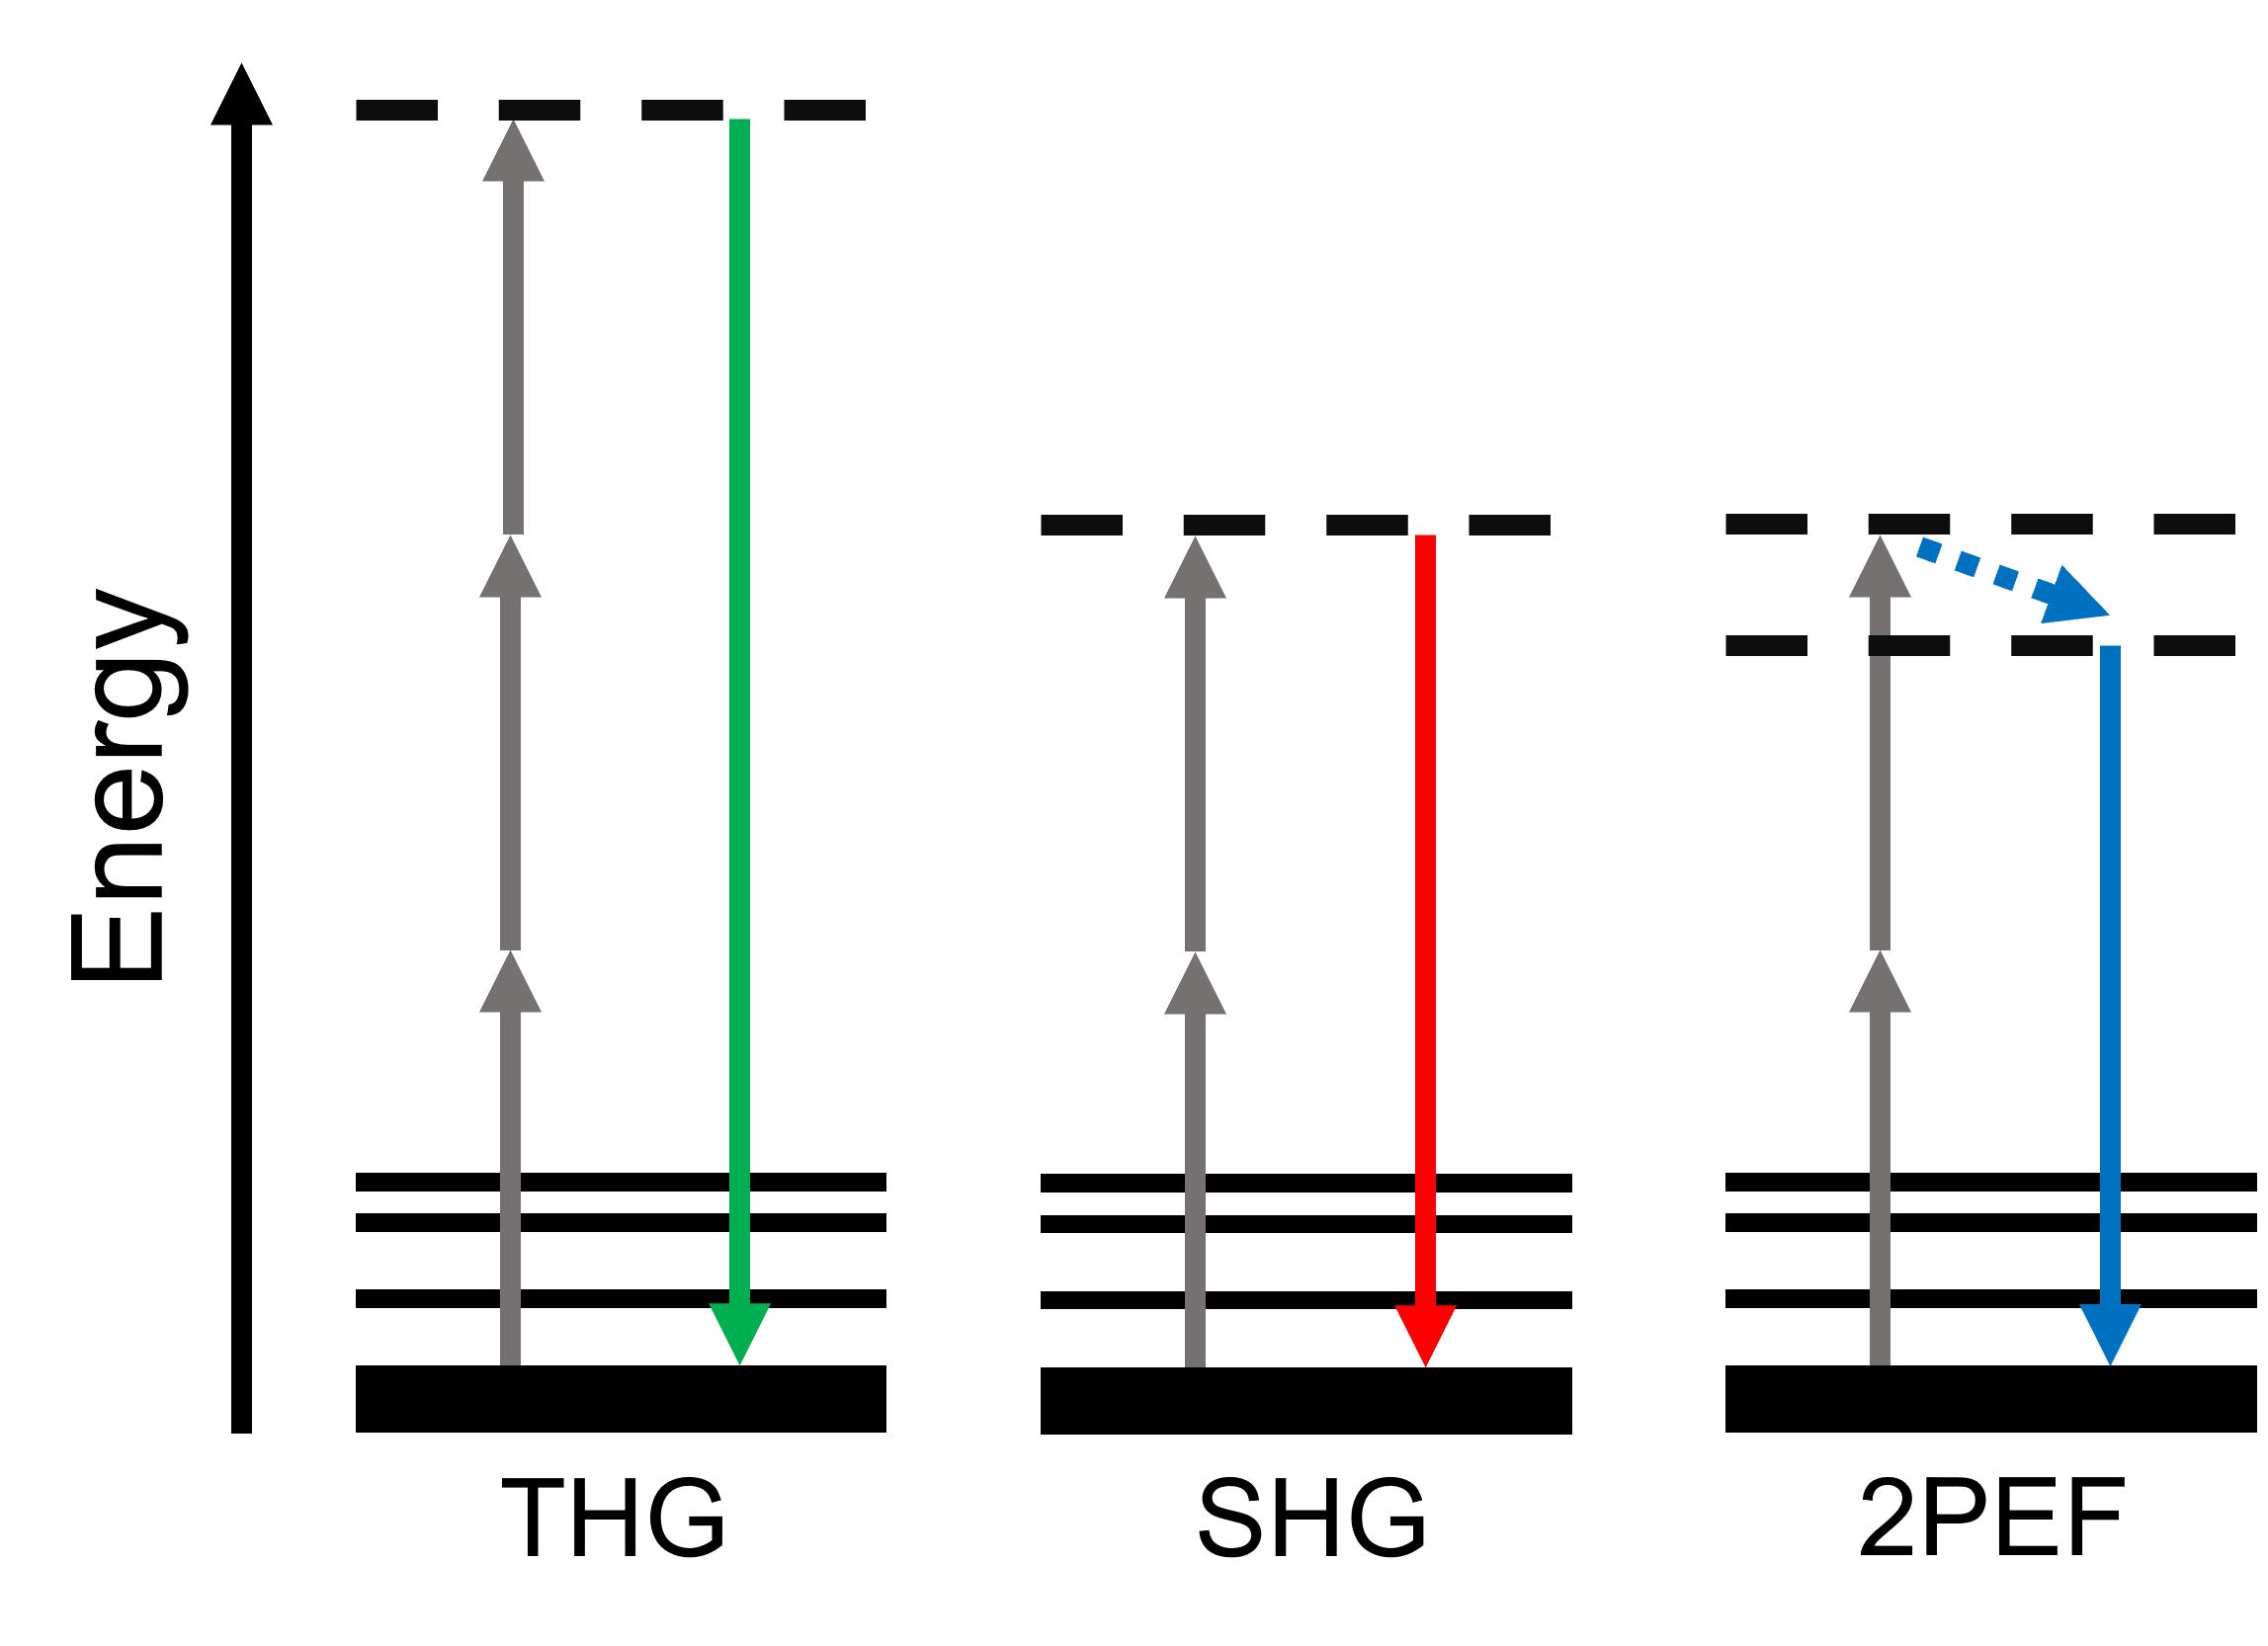
\includegraphics[width=\linewidth]{ANN/images/hhg-jablonski.png}
    \caption[THG, SHG and 2PEF Jablonski diagrams]{Jablonski diagrams for third and second harmonic generation (THG and SHG, respectively), and two-photon excitation fluorescence (2PEF).}
    \label{fig:hhg-jablonski}
\end{figure}
